\documentclass[12pt]{article}

\usepackage[utf8]{inputenc}
\usepackage{latexsym,amsfonts,amssymb,amsthm,amsmath}
\usepackage{graphicx}
\usepackage{titling}
\usepackage{gensymb}

\setlength{\parindent}{0in}
\setlength{\oddsidemargin}{0in}
\setlength{\textwidth}{6.5in}
\setlength{\textheight}{8.8in}
\setlength{\topmargin}{0in}
\setlength{\headheight}{18pt}
\setlength{\headsep}{-30pt}
\newcommand{\overbar}[1]{\mkern 1.5mu\overline{\mkern-1.5mu#1\mkern-1.5mu}\mkern 1.5mu}
\author{Bryan Wang}

\setlength{\droptitle}{-4em}
\title{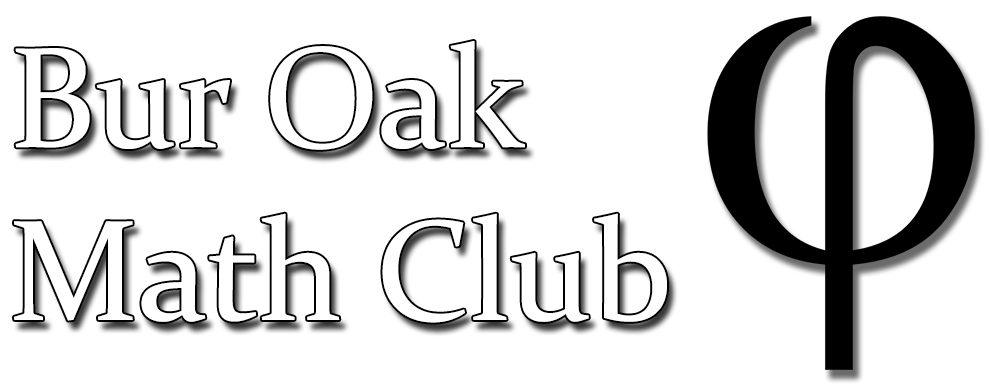
\includegraphics[width=10cm]{Bur Oak Math Club Banner Bold.png}\\\vspace{0.25in} Gr.11-12 Class 2 Homework (Quadrilaterals)}

\begin{document}
\maketitle

\subsection*{Exercise 1}
If \textit{ABCD} and \textit{EFGH} are squares and \textit{AB} = 1, find the area of the square \textit{EFGH}.
\begin{figure}[htp]
    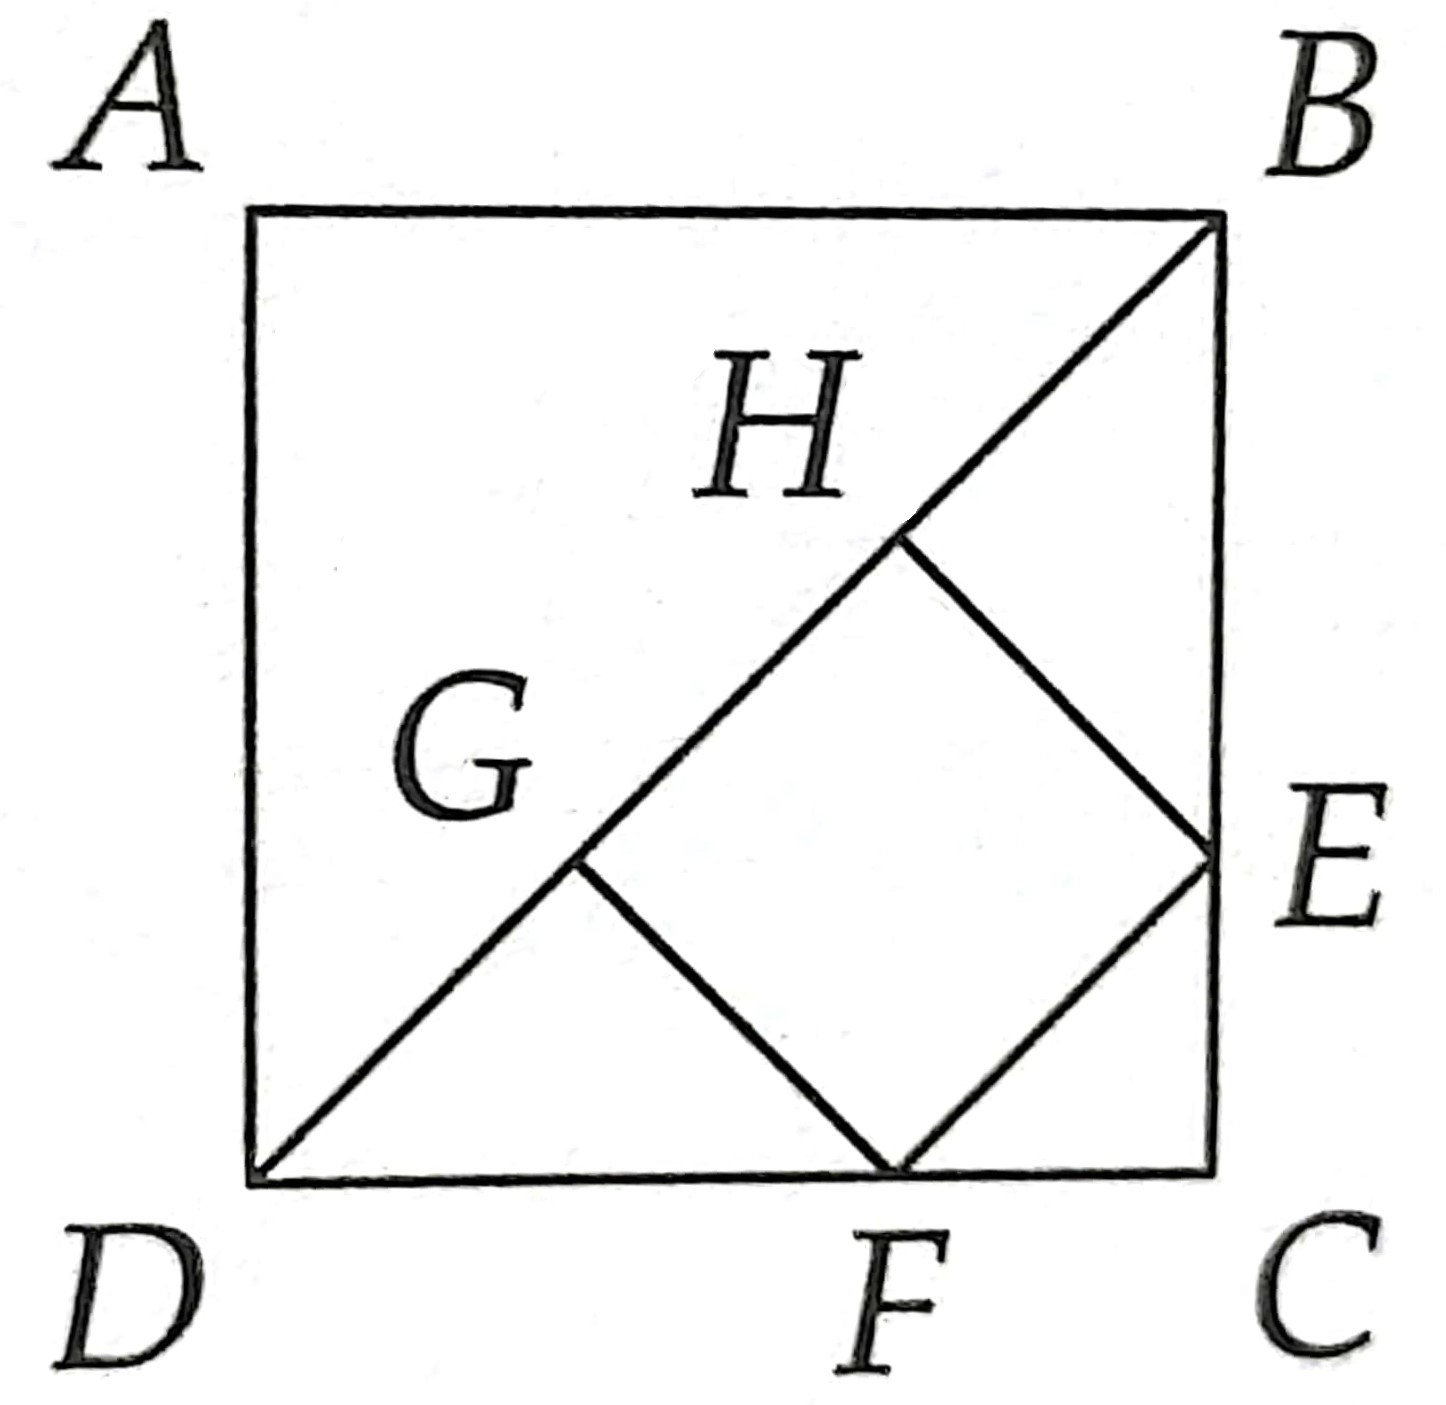
\includegraphics[width=6cm]{img2.jpg}
\end{figure}
\vspace{1.5in} %Leave space for comments!

\subsection*{Exercise 2}
What is the length of the common external tangent segment of two externally tangent circles whose radii are 8 and 11? (MA$\Theta$).
\vspace{3in} %Leave more space for comments!

\subsection*{Exercise 3}
Find the area of \textit{DUCK}.

\begin{figure}[htp]
    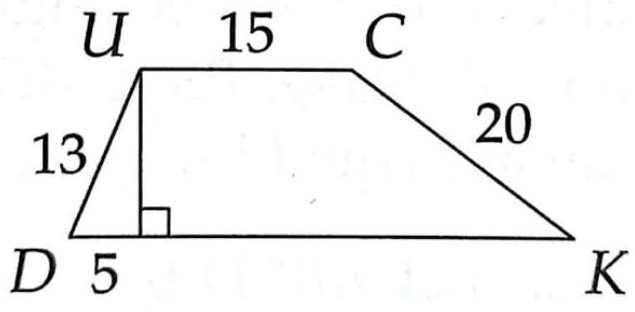
\includegraphics[width=6cm]{img3.jpg}
\end{figure}
\vspace{4in}


\subsection*{Exercise 4}
Given rectangle \textit{ABCD} such that \textit{AM} = \textit{MB}, \textit{AB} = 24, \textit{BC} = 18, and \textit{x} = \textit{DE}, find the value of \textit{x} such that the area of \textit{AMED} is exactly twice that of region \textit{MBCE}.

\begin{figure}[htp]
    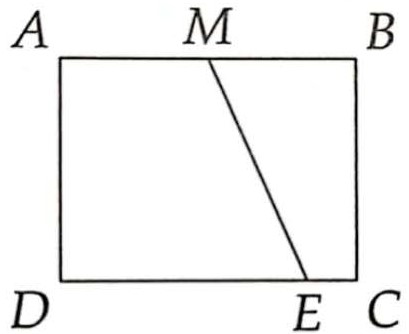
\includegraphics[width=5cm]{img4.jpg}
\end{figure}
\vspace{1.5in}

\subsection*{Exercise 5}
Quadrilateral \textit{ABCD} with consecutive sides of 8, 25, and 12 is inscribed in a circle with circumference 17$\pi$. Given that \textit{AC} is a diameter of the circle, what is the length of the other diagonal of the quadrilateral? (MA$\Theta$).
\vspace{3in}

\begin{center} 
\subsection*{Challenge Problems}
\end{center} 


\subsection*{Exercise 6}
Let \textit{ABCD} be a parallelogram of area 10 with \textit{AB} = 3 and \textit{BC} = 5. Locate \textit{E}, \textit{F}, and \textit{G} on segments \textit{AB}, \textit{BC}, and \textit{AD}, respectively, with \textit{AE} = \textit{BF} = \textit{AG} = 2. Let the line through \textit{G} parallel to \textit{EF} intersect \textit{CD} at \textit{H} Find the area of the quadrilateral \textit{EFHG}. (AHSME).
\vspace{3in}


\subsection*{Exercise 7}
Once upon a time, Ptolemy let his pupil draw an equilateral triangle $\Delta$ABC inscribed in a circle, before the great mathematician. He also added point \textit{D} and joined the red lines with other vertices, as shown. Unfortunately, they did not consider the advent of black and white printers. Regardless, they continue with their conversation:
\\
\\
\textbf{Ptolemy:} Dost thou see that all the red lines have the lengths in whole integers?
\\
\textbf{Pupil:} Indeed, master! Such an extraordinary point!
\\
\textbf{Ptolemy:} Now if the equilateral triangle has a side length of 13, what is the sum of the three red lengths combined?

\begin{figure}[htp]
    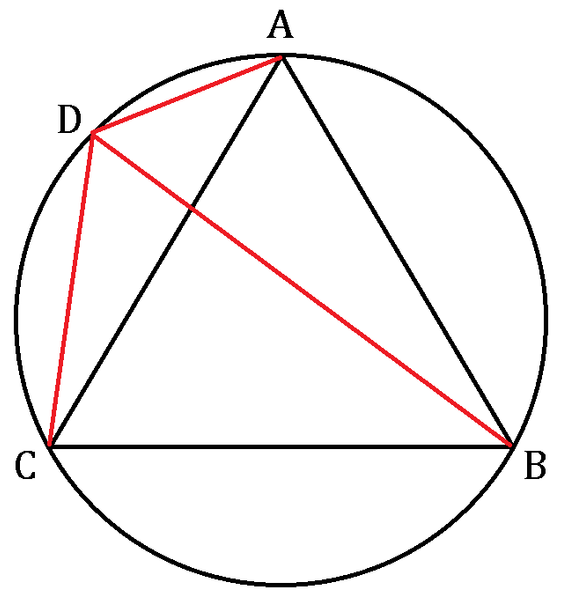
\includegraphics[width=9cm]{img1.png}
\end{figure}
\vspace{2in}


\end{document}
